
%|-----------------------------|
%| Description of merger trees |
%|-----------------------------|
\subsection{Merger trees}
\label{subsection:merger_trees}
As galaxies rarely evolve in isolation, they are subject to mergers with
neighbouring galaxies.  This adds serious complexity to tracing the history of
an individual galaxy from the present-day to its formation and as such we must
construct a \emph{merger tree} to connect galaxies across simulation output
times. Descendant subhaloes and hence galaxies are identified using the \dtrees
algorithm \citep{Jiang2014}, with a complete description of its adaptation to
the \eagle simulations provided in Qu et al. (\textit{in prep.}). In essence,
the algorithm traces subhaloes using the $N_{\text{link}}$ most bound particles
of any species, identifying the subhalo that contains the majority of these
particles as a subhalo's descendant at the next output time.  We define $N_{\rm
  link} = \min(100, \max(0.1N_{\rm galaxy}, 10))$, where $N_{\rm galaxy}$ is the
total number of particles in the parent subhalo.  This allows the identification
of descendants, even in the case where most particles have been stripped and it
minimises the misprediction of mergers during fly-bys \citep{Fakhouri08,
  Genel09}.

The galaxy with the most $N_{\rm link}$ particles at the next output is
identified as the single \emph{descendant} of a galaxy, while a descendant
galaxy can have multiple progenitors. The trees are stored in memory following
the method introduced by \cite{Lemson2006a} for the \emph{Millennium Simulation}
\citep[See also the supplementary material of][where the details of the tree
  ordering are summarized]{Springel2005b}. However, the
\emph{main progenitor}, corresponding to the main branch of the tree, is defined
as the progenitor with the largest \squotes{branch mass}, i.e., the mass summed
across all earlier outputs as proposed by \cite{DeLucia_Blaizot2007}. This
definition of the main progenitor, as opposed to the simple definition of the
progenitor with the largest mass, is used to avoid main branch swapping in the
case of similar-mass mergers, as explained by Qu et al. (\textit{in
  prep.}). Note that because the progenitor with the largest branch mass
determines the main branch of the tree, main branch galaxies do not necessarily
correspond to the central galaxy (or \texttt{SubGroupNumber} $= 0$ galaxy) of a
given halo.

There are two further aspects of the merger trees that must be kept in mind when
analysing the simulation:
\begin{itemize}

\item A galaxy can disappear from a snapshot but reappear at a later time
  (e.g. if one galaxy passes through another one).  To account for this,
  descendants are identified using up to 5 snapshots at later times.

\item Care must be taken when determining mass ratios, for example in the case
  of mergers, as galaxies can lose or gain mass due to the definition of the
  subhaloes.
\end{itemize}

Both of these relatively rare cases are considered further by Qu et
al. (\textit{in prep.}), who discuss their impact on the assembly of galaxy
mass.\\

\begin{figure*}[t]
\centering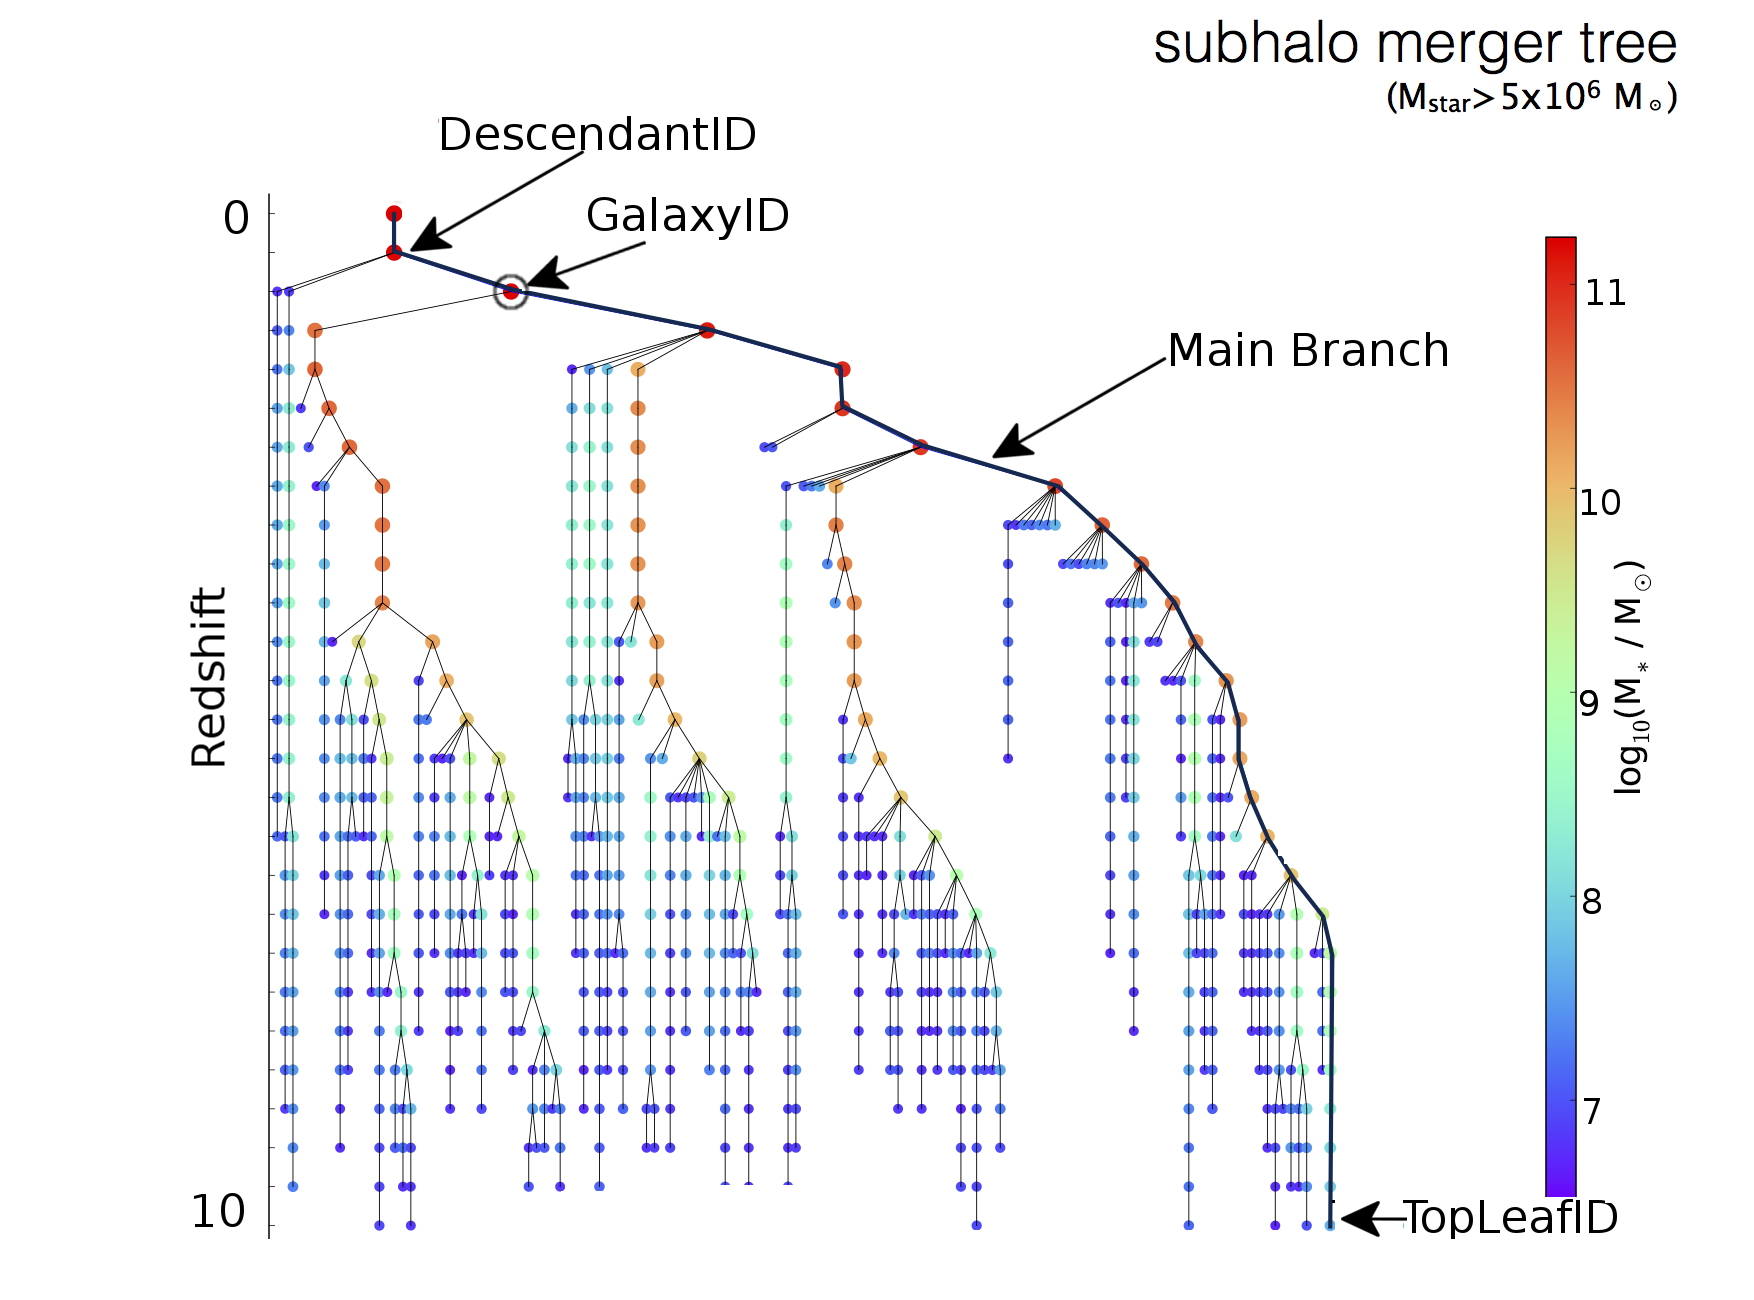
\includegraphics[width=\textwidth]{figures/nam_tree_ex.png}
\caption{Merger history of a galaxy with a $z=0.18$ stellar mass M$_*\sim10^{10}
  \Msol$ indicated by the circled dot. Symbol colours and sizes are scaled with
  the logarithm of the stellar mass. The \HaloID of this galaxy points towards
  it, as indicated by the arrow. The main progenitor branch is indicated with a
  thick black line, all other branches with a thin line. The \TopLeafID gives
  the \HaloID of the highest redshift galaxy on the main progenitor branch
  whilst the \LastProgID (not shown) gives the maximum \HaloID of all the
  progenitors of the galaxy considered. Querying all galaxies with an ID between
  \GalaxyID and \LastProgID will return all the progenitor galaxies in the
  tree.}
\label{fig:mergerTree}
\end{figure*}

